This section presents a comparative analysis of the performance of three distinct websites. To gain insights into their performance under different 
conditions, two key parameters (Figure \ref{fig:4_tuples}) were varied throughout the experiments: the number of requests sent to each website and the concurrency level. 
It is important to note that these parameters' values were chosen conscientiously, taking ethical considerations into account to prevent overloading the websites.
All experiments were conducted using identical conditions, as described in Section \ref{sec:experimental_setup}. The used scripts
can be consulted in Appendix \ref{sec:scripts}.

    \begin{figure}[H]
        \centering
        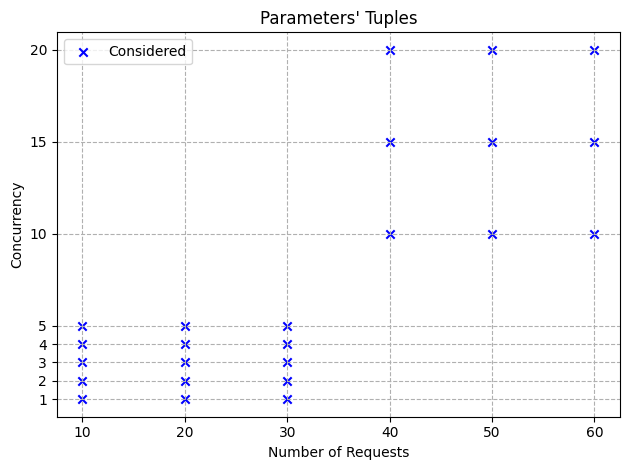
\includegraphics[width=0.48\textwidth]{4_tuples.png}
        \caption{\small Concurrency and RPS combinations}
        \label{fig:4_tuples}
    \end{figure}



It is worth mentioning 
that the client-side cache was intentionally disabled to ensure that the experiments accurately captured the website's performance without any caching effect.
All the results were gathered using the \textit{Apache Benchmark} tool, and the metric used to compare the websites is the RPS (Requests Per Second).
Three analysis are presented: the first one consider the impact on the RPS of the concurrency level, the second one the impact of the number of requests,
and the last the overall RPS achieved by each website.

\subsubsection{Concurrency VS RPS}
The concurrency is intended as the number of concurrent clients hitting the website at the same time. As the concurrency level increases, 
the website's server is required to process multiple requests concurrently. This can result in a higher 
RPS, as more requests are being handled simultaneously. However, there may be limits to the server's capacity 
to handle concurrent requests efficiently.
If the server is properly configured and equipped to handle the increased concurrency, it may exhibit a linear or near-linear increase in 
RPS as the concurrency level rises. 
However, there may be a point of diminishing returns where further increasing the concurrency level does not lead to a significant increase 
in RPS or may even negatively impact the server's performance. This can occur if the server becomes overwhelmed with the high concurrency, 
leading to delays and increased response times. The results in Figure \ref{fig:4_web_conc} depict the RPS (averaged across number of requests)
for each tuple (website, concurrency level). The Requests Per Second increase with the concurrency in a less than linear way until a 
threshold (10 in this case). After that point, 'MIT' and 'Apple' showed some performance degradation, suggesting they might start
struggling to handle the increased concurrency. 'Harvard' instead, showed a constant increasing trend. It is worth to mention that the 
RPS values are influenced by many other factors, such as the server's load at the time of the experiment, that may have affected the results.

    \begin{figure}[H]
        \centering
        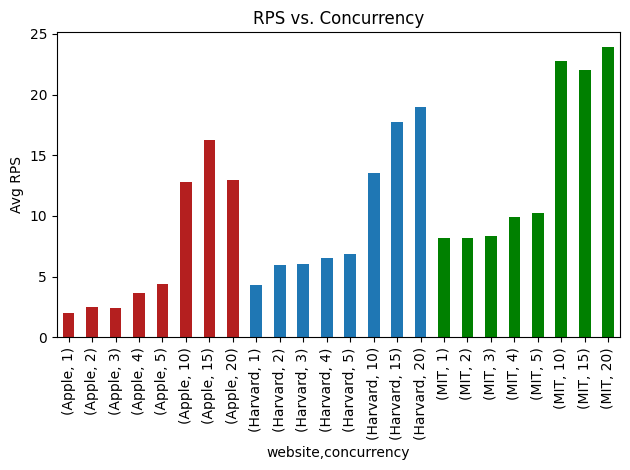
\includegraphics[width=0.48\textwidth]{4_web_conc.png}
        \caption{\small Concurrency VS RPS}
        \label{fig:4_web_conc}
    \end{figure}


\subsubsection{Number of requests VS RPS}
The number of requests sent to a website in a given time interval is another important factor that can affect the website's performance.
As the number of requests increases, the server is forced to handle an higher volume of traffic and the considerations about the 
RPS behavior may not change from the ones discussed above. The results in Figure \ref{fig:4_web_num} show the RPS (averaged across concurrency level)
for each tuple (website, number of requests). As expected there is a positive correlation between the number of requests and the RPS, with the websites
'Apple' and 'MIT' showing a trend quite similar to the one observed in the concurrency analysis. 'Harvard' instead, shows an odd behavior with 
50 requests. According to Figure \ref{fig:4_detailed}, the justification is a dip in the RPS value for 50 requests and 10 concurrency level.
The reasons for this behavior are not clear, therefore a further investigation is necessary.\\

    \begin{figure}[H]
        \centering
        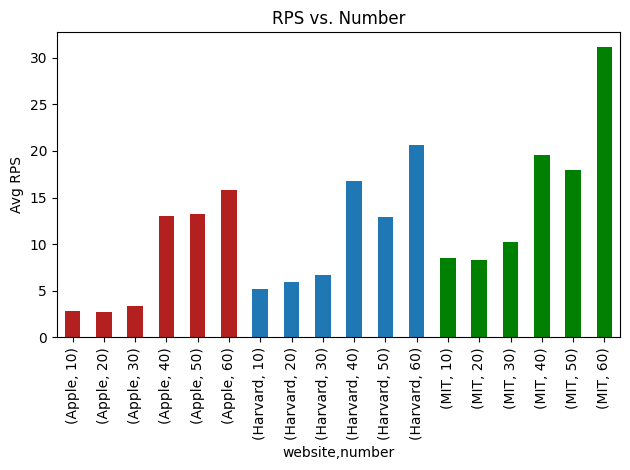
\includegraphics[width=0.48\textwidth]{4_web_num.png}
        \caption{\small Number of requests VS RPS}
        \label{fig:4_web_num}
    \end{figure}

\subsubsection{Overall RPS}
In conclusion to asses a overall performance of the websites, the RPS values for each website were averaged across all the concurrency levels and
number of requests. The results are shown in Figure \ref{fig:4_overall}. The website achieving the highest average RPS is 'MIT', followed by 'Harvard'
and 'Apple'.

    \begin{figure}[H]
        \centering
        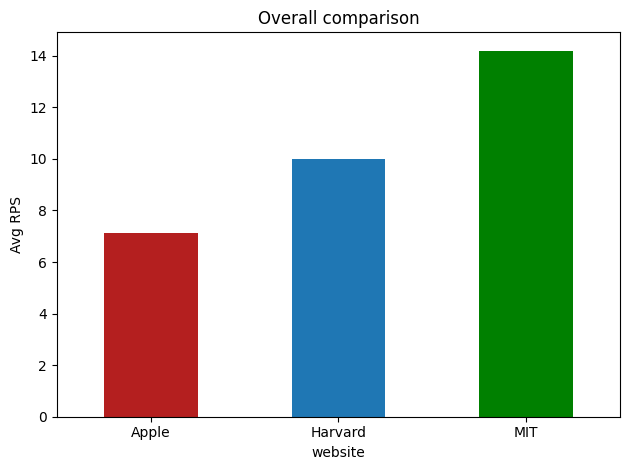
\includegraphics[width=0.48\textwidth]{4_overall.png}
        \caption{\small Overall RPS}
        \label{fig:4_overall}
    \end{figure}

